% ==================================
%            Chapter 3.4
%         Linear Inequalities
%       Created by Michael Tang
%             2025.02.25
% ==================================

\subsection{Linear Inequalities}
\begin{itemize}
    \item \textbf{Key Concept:} A linear inequality is similar to a linear equation, but instead of an equal sign, we have an
    inequality sign ($<$, $\leq$, $>$, $\geq$). The solution is the set of real numbers that satisfy the inequality.
    \item \textbf{Methods for Solving Linear Inequalities}
    \begin{itemize}
        \item Rearrange the inequality to isolate the variable on one side.
        \item Solve as would for an equation.
        \item Check the direction of the inequality when multiplying or dividing by a negative number, as this reverses the
        inequality sign.
    \end{itemize}
    \item \textbf{\underline{Set Notation} (集合计数法) for Solutions}
    \begin{itemize}
        \item For inequalities like $x \geq 2.75$, write in set notation as $\{x : x \geq 2.75\}$.
        \item For compound inequalities (e.g., $x > -1$ and $x \leq 4$), write as $\{x : -1 < x \leq 4\}$.
    \end{itemize}
    \item \textbf{Graphical Representation}
    \begin{figure}[H]
        \centering
        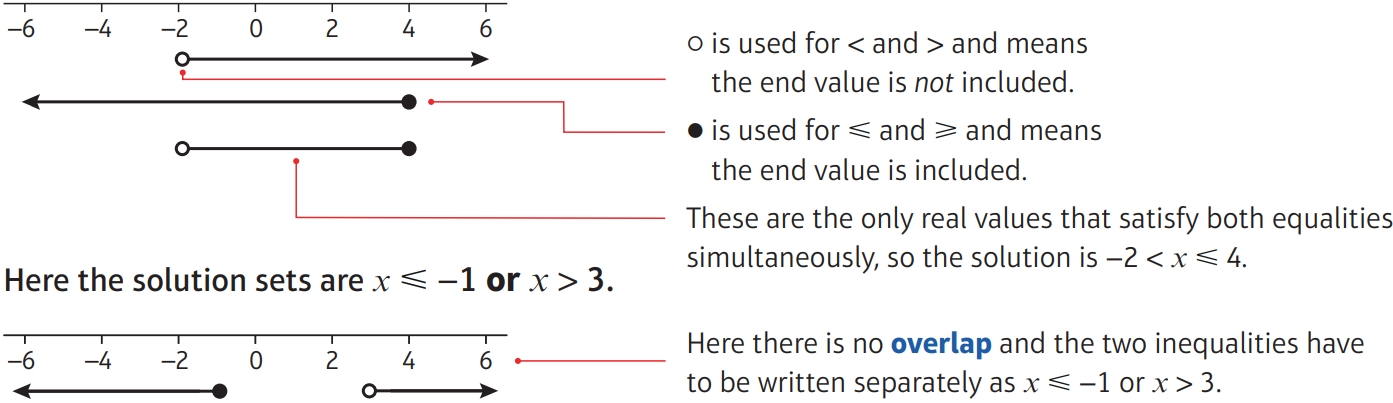
\includegraphics[scale=0.2]{Mathematics/Pure Mathematics/Ch3/Images/Ch3-4-1.png}
    \end{figure}
\end{itemize}